\chapter{Planteamiento del Problema}

Las redes de monitoreo de meteorológico y de calidad del aire de alta densidad son una necesidad creciente de las áreas urbanizadas, las cuales necesitan de una infraestructura cada vez más compleja para su monitoreo y mantenimiento. Estas necesidades crecientes de infraestructura han generado una demanda creciente de recursos humanos, y la falta de homogeneidad entre las estaciones de monitoreo presentan retos a conquistar para proveer servicios cada vez más sofisticados. En este capítulo, se discutirá la importancia de la infraestructura de monitoreo y se explicarán los diferentes métodos de realizarlo que son utilizados actualmente para monitorear las estaciones meteorológicas, así como una propuesta de solución para los problemas que los sistemas tradicionales existentes presentan.

\section{Antecedentes}

El desplegar y mantener una red meteorológica urbana compone bastantes retos: Entre la creciente dificultad de crear sistemas de medición estandarizados que se adapten al siempre cambiante paisaje urbano; como la instalación de los equipos de medición y de guardado de datos en áreas que permitan acceso para mantenimiento y que sean seguros; y la dificultad de encontrar un punto de acceso a internet adecuado para transferir la información generada, el generar una red de monitoreo es una tarea extensa y compleja.

Debido a estos retos, la comunidad de monitoreo climatológico y meteorológico se ha enfocado en la creación de sistemas que sean más eficientes y económicos. Entre estos esfuerzos, se encuentra el amplio uso de dispositivos RaspberryPi como centro de recolección de datos de estaciones de monitoreo \cite{rpi_weataher_station}, tanto caseras como profesionales, con la ayuda de sistemas abiertos para la recolección de datos como lo es WeeWX. Esto ha hecho factible el desplegar redes de 50 nodos de monitoreo con sensores económicamente viables para actores con un presupuesto limitado \cite{monitoreo_raspberry_nagios}.

% TODO! Agregar sección de monitoreo de Campbell, y como funciona actualmente. Port forwarding en Campbell, porque no están en nuestra red.

%! Davis Weatherlink Live. https://www.davisinstruments.com/weatherlinklive/

Estas redes densas requieren de un monitoreo continuo para mantener una alta calidad de los datos recabados, y así evitar las pérdidas por falta de mantenimiento. Entre los sistemas de monitoreo que pueden ser adaptados para el monitoreo de estaciones meteorológicas y la red que las soporta, se encuentra la plataforma Nagios, la cual es un sistema de monitoreo continuo orientado a redes y servidores. Entre la información que recaba Nagios contínuamente para el estado de los servidores, se encuentra el uso de CPU y RAM, así como estado de los discos, puertos, e información variada de servicios de red en los hosts. Debido a que Nagios es un sistema de monitoreo de redes orientado a profesionales de la informática, la interfaz gráfica es poco amigable con los usuarios menos familiarizados con los conceptos técnicos de los sistemas computacionales, como se muestra en la Figura \ref{fig:nagios_dashboard}.

\begin{figure}[!ht]
	\centering
	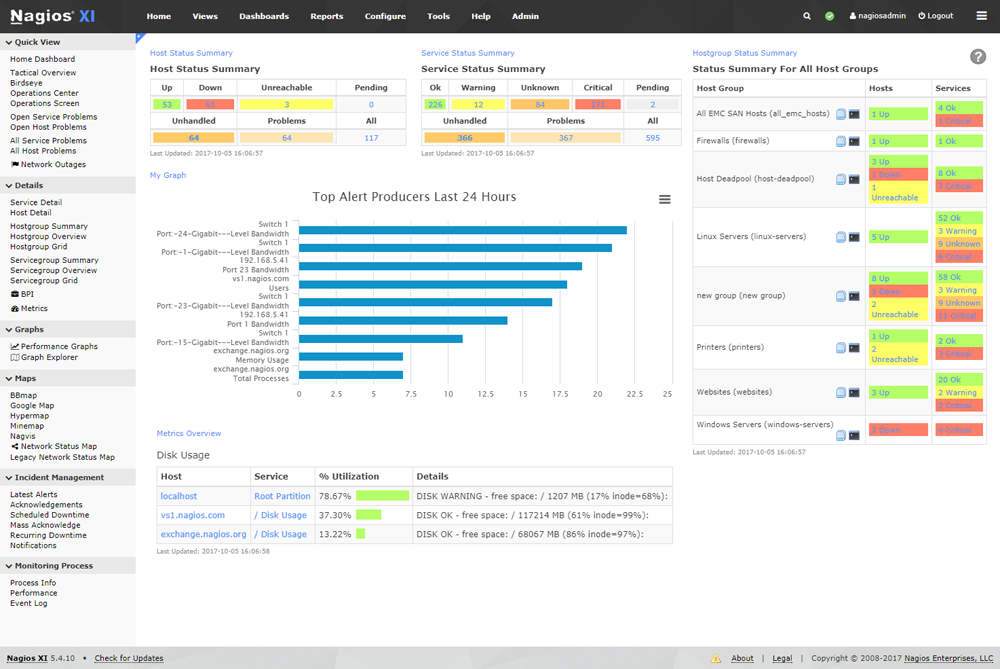
\includegraphics[width=1\linewidth]{images/Nagios_home_dashboard.png}
	\caption{Tablero principal de Nagios XI.}
	\label{fig:nagios_dashboard}
\end{figure}

Aunque Nagios ofrece la posibilidad de monitorear parámetros adicionales y posee una comunidad establecida que desarrolla continuamente en diversos lenguajes, como Python, un sistema conformado por plugins relacionados con el proyecto. Sin embargo, la cantidad de éstos relacionados con estaciones meteorológicas existentes es mínima ya que los esfuerzos de la comunidad se centran principalmente en el monitoreo de centros de datos, redes y routers.

Además de los plugins existentes en la comunidad de Nagios, existe la alternativa abierta conocida como \textit{monitoring plugins} \cite{monitoring_plugins}, que es una plataforma compatible con diversos sistemas de monitoreo de redes y servicios, en la cual es posible encontrar una mayor cantidad de scripts de monitoreo relacionados con los sistemas de recolección de datos meteorológicos. La utilización de estos \textit{plugins abiertos} junto con un sistema central como Nagios ya ha sido propuesto anteriormente, sin embargo, se descartó un monitoreo más profundo debido a que \say{las métricas obtenidas son muy simples y los valores se devuelven de comandos directos de sistema de GNU/Linux} \cite{monitoreo_raspberry_nagios}.

Las limitaciones de Nagios vienen a raíz de su implementación orientada a sistemas de alta disponibilidad y el generalismo en la implementación de monitoreo, la configuración de los parámetros de tolerancia para la resilencia a fallas son generalmente limitados en la variedad de los mismos y los valores fijos que se pueden establecer. Además, debido a las necesidades de seguridad y accesibilidad de las estaciones meteorológicas en el contexto urbano, estas suelen instalarse en sistemas en los que se posee poco control de la red que les provee comunicación, como son las escuelas, hospitales y estaciones de policía, así como otros espacios públicos \cite{muller_sensors_and_the_city}, dificultando aún más la capacidad de monitoreo y disponibilidad de la red y los sistemas que soporta. Esta limitante se hace más presente debido a que los sistemas se vuelven completamente dependientes de una VPN para funcionar y para su control, debido al extenso uso de redes IPv4 bajo NAT que predominan en los sitios de instalación.

Otra de las restricciones del sistema Nagios es que al ser un sistema de monitoreo limita la capacidad de acción de los usuarios ante un caso que lo requiera. Si bien es posible el realizar acciones por medio de scripts creados al momento de la configuración de Nagios, estos requieren una configuración extensa y compleja \cite{nagios_service_restart}. Además, el sistema basado en eventos impide la interacción directa de un usuario para la respuesta de forma directa desde la consola de administración, requiriendo que el usuario tenga un conocimiento del método de conexión, así como la información necesaria para realizar una tarea trivial como es el reiniciar un servicio.

Actualmente, el sistema de monitoreo de calidad del aire y climatológico del Centro Climatológico y de Calidad del Aire (CECATEV) en la Universidad Autónoma de Ciudad Juárez, engloba varios de los retos antes descritos, ya que a pesar de la baja densidad de estaciones meteorológicas, comprende una variedad importante de las mismas. Esta compuesta por prototipos conectados por medio de redes virtuales privadas, monitoreados remotamente \cite{red_climatologica_uacj}, estaciones de diferentes proveedores, siendo monitoreadas local y externamente, así como estaciones remotas con routers dentro de la red local de la universidad (véase la Figura \ref{fig:current_network}). Lo que provoca que sea un reto monitorearlas adecuadamente debido a la variedad de sus componentes.

%* Los puertos no están expuestos si la conexión se realiza por NAT.

%! (Centro de Ciencias Atmosféricas y Tecnologías Verdes)

\begin{figure}[!ht]
	\centering
	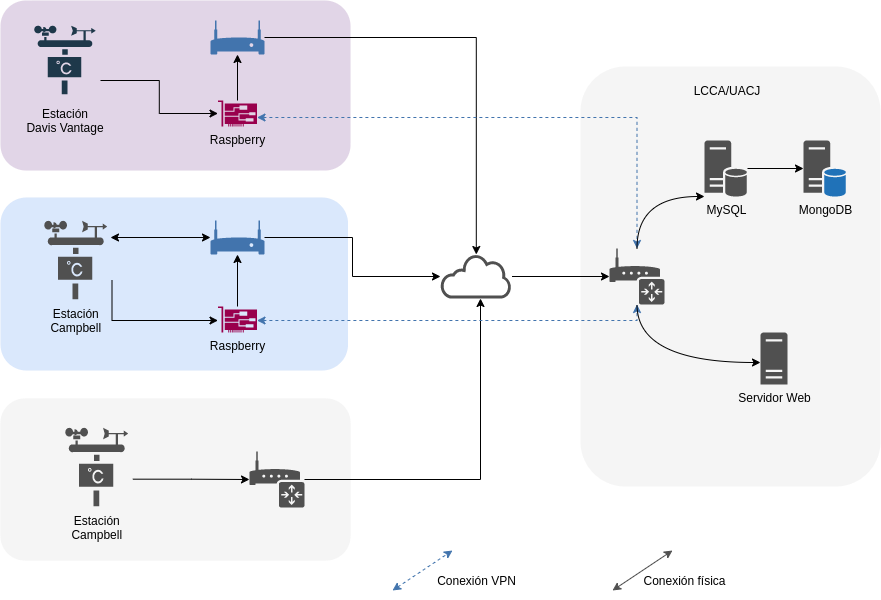
\includegraphics[width=.80\linewidth]{images/diagrams/red_lcca.drawio.png}
	\caption{Diagrama de red de CECATEV UACJ.}
	\label{fig:current_network}
\end{figure}

Desafortunadamente, la infraestructura de la red actual del LCCA no cuenta con un sistema de monitoreo para el registro automático de problemas de las estaciones meteorológicas de la cual pueda ser derivada información de la calidad de los datos meteorológicos así como un estado de salud de las estaciones. Esto, dificulta el uso de forma adecuada de la información existente e impide la generación de reportes de calidad de la información.

\section{Definición del problema}

La falta de una plataforma estandarizada para el monitoreo de estaciones meteorológicas que permita un monitoreo continuo y control de diversos tipos de estaciones, así como la disponibilidad del acceso a los datos, y un registro de incidentes crea una dificultad creciente para los administradores de redes de monitoreo meteorológico. Con redes cada vez más densas que son más accesibles económicamente y menos complejas de crear, se hace notar la necesidad de un sistema estandarizado y compatible con soluciones existentes para el monitoreo de las estaciones.

\section{Objetivo general}

Desarrollar un sistema de monitoreo y control de estaciones meteorológicas para personal no especializado, capaz de proveer datos y herramientas que coadyuven en el mantenimiento preventivo y correctivo de las mismas.

\subsection{Objetivos específicos}

\begin{itemize}
   \item Desarrollar un sistema central para coordinar y recolectar los datos del estado de las estaciones.

   \item Diseñar un API REST para consultar el estado de las estaciones meteorológicas.

   %! Agregar como subobjetivo una base de conocimientos. (como lo justifico?) Demostrar tiempos de respuesta para QAPP.
   %! Herramientas de gestión de calidad
   %! Personas como parte de gestion

   \item Diseñar e implementar una interfaz gráfica para monitorear el estado de las estaciones.

   \item Integrar las diferentes estaciones meteorológicas existentes al sistema creando los controladores correspondientes.

   \item Integrar un sistema existente de notificaciones/alertas de terceros para fallos críticos de las estaciones.
\end{itemize}

\section{Justificación}

Creando un sistema de monitoreo eficaz para las estaciones meteorológicas se pretende el alcanzar una mayor calidad de los datos obtenidos de las mismas, así como una mejor documentación por consecuencia de los problemas de los sistemas meteorológicos. Esto pretende dar el tiempo al personal especializado en enfocarse en expandir las redes existentes meteorológicas, mejorando a largo plazo la calidad y la definición de los datos recabados con la misma cantidad de esfuerzo.

Además, haciendo el sistema de monitoreo un proyecto público y compatible con soluciones existentes, se pretende el ayudar a mejorar la calidad y confiabilidad de las redes de monitoreo meteorológico, de calidad del aire y climatológico al rededor del mundo.

Este proyecto tiene un impacto tecnológico, debido a que se plantea el desarrollar un sistema en el que se puedan integrar diversos datos que ayuden a generar un estado comprehensible de la calidad de la información de las redes meteorológicas que monitorea. Con respecto al impacto económico, el proyecto le permitirá identificar y solucionar los problemas que ocurrieran en las diferentes estaciones sin la  necesidad de desplazarse para corregir la solución, propiciando un uso más eficiente de los recursos humanos y económicos de CECATEV cuyo financiamiento principal para la operación son recursos públicos.

El impacto ecológico del proyecto es indirecto ya que el personal de CECATEV podrá dedicar mayor tiempo al tratamiento de la información generada por las estaciones y no en desplazarse a las diferentes estaciones para identificar los problemas y solucionarlos.

\section{Alcances y limitaciones}

\noindent Entre los alcances que se pretendían lograr con el proyecto, se contemplaron los siguientes:

\begin{itemize}

   \item Se integraron estaciones meteorológicas existentes, que se encontraban conectadas a la red de comunicaciones del CECATEV ya sea directamente o por medio de una VPN.

   \item Se entregó un sistema instaldo, funcional y listo para monitorear las estaciones seleccionadas, sin necesidad de configuraciones extraordinarias.

\end{itemize}

Si bien se pretende que el proyecto tenga la flexibilidad suficiente para adaptarse a nuevos casos de uso sin necesidad  de reescribir grandes partes del mismo, también se consideran las siguientes limitaciones:

\begin{itemize}

\item La integración se limitó a cubrir casos conocidos y recurrentes de estaciones meteorológicas existentes.
\item Solo se considera integrar una estación meteorológica de cada tipo en cada topología, dejando como proyecto futuro integrar la totalidad de la red de la universidad.
\item El sistema se limita a cubrir los casos de fallas comunes y conocidos de las estaciones.
\item Sólo se monitorean los servicios básicos de las estaciones meteorológicas que son vitales para el funcionamiento.
\end{itemize}
